\chapter{Results}
\section{Babel Stream}\label{sec:res-babel}
Babel Stream's results show that Rust and Rayon are unable to scale as well as C++ and OpenMP\@. Figures~\ref{fig:babel-dot},~\ref{fig:babel-add} and~\ref{fig:babel-triad} all show that Rust and C++ have similar performance but that at higher thread counts, there is a great deal of difference between the threading performance of both implementations. In each figure, 1gb refers to the size of the single array in that execution run, and chunk\_xxMB refers to how large a subsection of that array the threads are assigned to.

For example, both Rust and C++ having very similar memory bandwidths in the Dot product's serial execution, with Rust at 11453 MB/s and C++ at 11563 MB/s, giving a difference in bandwidth of just 1\%.\todo{replace with sig figs?}
However, this difference later widens at 32 threads to 35\% with Rust at 87336 MB/s and C++ at 135106 MB/s

\begin{figure}[h]
\centering
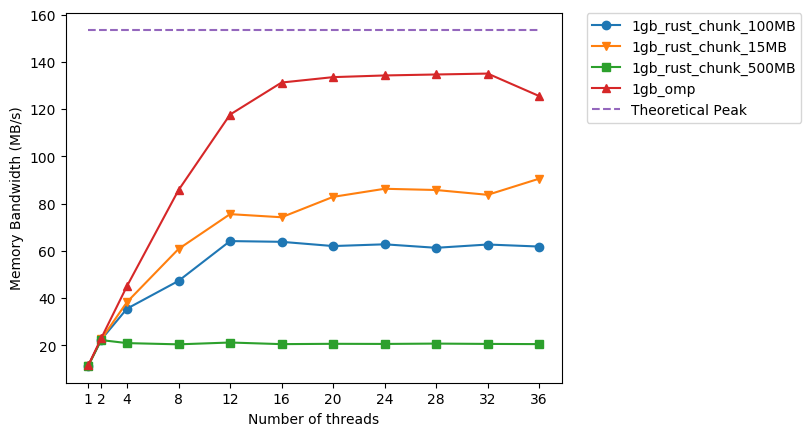
\includegraphics[width=.9\linewidth]{figs/babel/Dot.png}
\caption{Babel Stream --- Dot product bandwidth}\label{fig:babel-dot}
\end{figure}

Whilst the performance difference is not so pronounced for both the add and triad benchmarks, shown in Figure~\ref{fig:babel-add} and~\ref{fig:babel-triad} it is still quite promininent, with a performance difference of \% for add and \% for triad. It is interesting that the dot product is able to attain such a higher level of memory bandwidth. Although a deep investigation into why the dot product attains a higher bandwidth than the add or triad benchmarks, I believe likely due to the hardware's implementation of combined operationl units, like fused multiply adds, as a cursory inspection of the assembly code here did not reveal any sufficent optimisations at that level.

\begin{figure}[h]
\centering
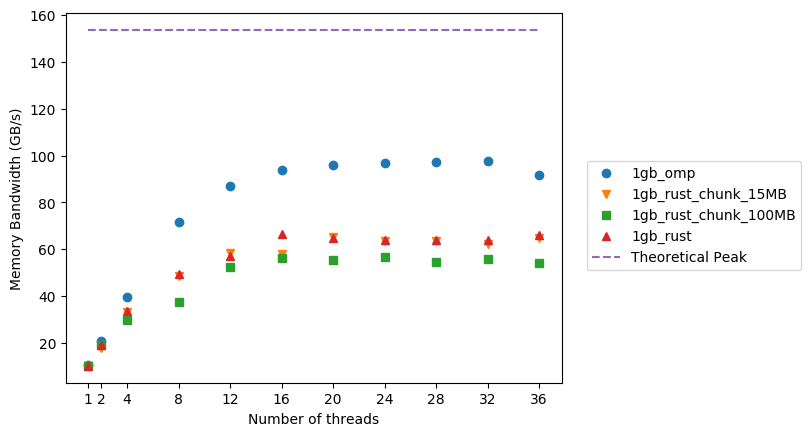
\includegraphics[width=.9\linewidth]{figs/babel/Add.png}
\caption{Babel Stream --- Add bandwidth}\label{fig:babel-add}
\end{figure}

This increasing difference lead me to believe that an examination of assembly code would not be beneficial in this circumstance, as it seemed like the low level, assembly implementation of both of the dot product was not that different. Instead, it seemed like the threading implementation was so different that it was what was causing the problem, which is much easier to understand in its high level expression. I decided to investigate the thread scheduling implemtation.

\begin{figure}[h]
\centering
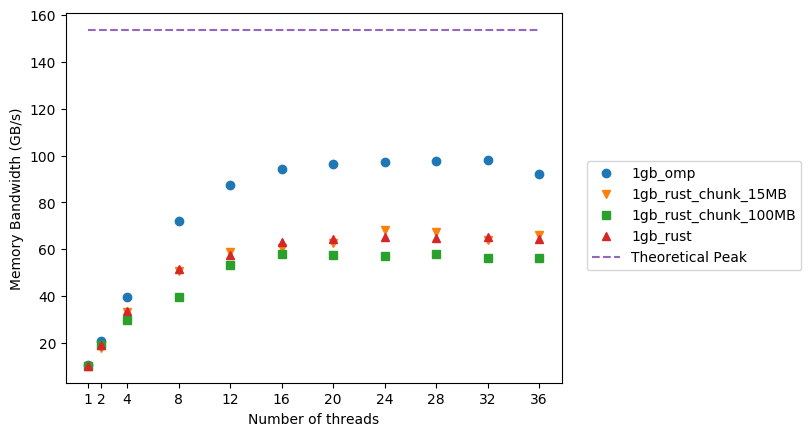
\includegraphics[width=.9\linewidth]{figs/babel/Triad.png}
\caption{Babel Stream --- Triad bandwidth}\label{fig:babel-triad}
\end{figure}

The decision to investigate thread scheduling was made because it was easy to investigate. There was also the possiblity that Rayon's context switching was more costly to perfromance than OpenMPs.
\section{Sparse Matrix}\label{sec:res-sparse}
\section{K-means}
\section{Questionnaire}
